\documentclass[a4paper,UTF8]{article}
\usepackage{ctex}
\usepackage[margin=1.25in]{geometry}
\usepackage{color}
\usepackage{graphicx}
\usepackage{amssymb}
\usepackage{amsmath}
\DeclareMathOperator*{\argmax}{argmax}
\usepackage{amsthm}
%\usepackage[thmmarks, amsmath, thref]{ntheorem}
\theoremstyle{definition}
\newtheorem*{solution}{Solution}
\newtheorem*{prove}{Proof}
\usepackage{multirow}
\usepackage{url}
\usepackage{enumerate}
\usepackage{algorithm}
\usepackage{algorithmic}
\usepackage{caption}
\usepackage{mathrsfs}
\renewcommand{\algorithmicrequire}{\textbf{Input:}}
\renewcommand{\algorithmicensure}{\textbf{Procedure:}}
\renewcommand\refname{参考文献}

%--

%--
\begin{document}
\title{实验2. 隐马尔科夫模型实践}
\author{MG1733079,杨佩成,\url{18362903155@163.com}}
\maketitle

\section*{综述}
	隐藏马尔科夫模型(Hidden Markov Model)是一种著名的有向图模型,主要用于时序数据建模,在语音识别、自然语言处理等领域有广泛应用\cite{reference1}。
\begin{figure}[h]
\centering
\small
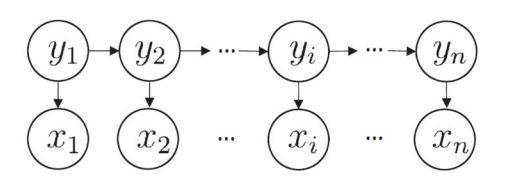
\includegraphics{1.JPG}
\caption{隐马尔科夫模型的图结构}
\end{figure}

	如Figure 1所示,隐马尔科夫模型中的变量可分为两组。第一组是状态变量 $\left\{ y_1,y_2,...,y_n\right\}$,其中$y_i \in \mathcal{Y}$表示第i时刻的系统状态。通常状态变量是隐藏的、不可被观测的,因此状态变量也叫隐变量。第二组是观测变量$\left\{ x_1,x_2,...,x_3 \right\}$,其中$x_i \in \mathcal{X}$表示第i时刻的观测值。
	
	Figure 1中的箭头表示了变量间的依赖关系。在任意时刻,观测变量仅依赖于状态变量。同时,$t$时刻的状态$y_t$仅依赖于$t-1$时刻的状态$y_{t-1}$。基于这种依赖关系,所有变量的联合概率分布为
\begin{displaymath}
	P(x_1,y_1,...,x_n,y_n)=P(y_1)P(x_1|y_1)\prod_{i=2}^nP(y_i|y_{i-1})P(x_i|y_i).
\end{displaymath}

	除了结构信息,要确定一个隐马尔科夫模型需要以下三组参数:
\begin{itemize}
\item
	状态转移概率:模型在各个状态间转换的概率,通常记为矩阵$\textbf{A}=[a_{ij}]_{N\times N}$,其中
\begin{displaymath}
	a_{ij}=P(y_{t+1}=s_j|y_t=s_i),\qquad 1 \leq i,j \leq N,
\end{displaymath}
表示在任意时刻$t$,若状态为$s_i$,则下一时刻状态为$s_j$的概率。
\item
	输出观测概率:模型根据当前状态获得各个观测值的概率,通常记为矩阵$\textbf{B}=[b_{ij}]_{N\times M}$,其中
\begin{displaymath}
	b_{ij}=P(x_t=o_j|y_t=s_i),\qquad 1 \leq i \leq N, 1\leq j \leq M
\end{displaymath}
表示在任意时刻$t$,若状态为$s_i$,则观测值$o_j$被观测的概率。
\item
     初始状态概率:模型在初始时刻各个状态出现的概率,通常记为$\boldsymbol{\pi}=(\pi_1,\pi_2,...,\pi_N)$,其中
\begin{displaymath}
	\pi_i=P(y_1=s_i),\qquad 1\leq i \leq N
\end{displaymath}
表示模型的初始状态为$s_i$的概率。
\end{itemize}

	通过指定状态空间$\mathcal{Y}$、观测空间$\mathcal{X}$和上述三组参数,就可以确定一个隐马尔科夫模型。在本次实验中,我们使用HMM对股票数据进行分析和预测。对于单只股票,我们可以观察到的值可以是涨、跌、不涨不跌。我们假设股票的涨跌由内在的隐变量驱动,即牛市或熊市。

\section*{实验一.}
	实验一我们对训练好的HMM,利用维特比算法对模型进行推断。维特比算法是一种使用动态规划思想来寻找最有可能的隐状态序列的算法,维特比算法的基础可以概括为以下三点\cite{reference2}:1、 如果概率最大的路径经过篱笆网络的某点,则从开始点到该点的子路径也一定是从开始到该点路径中概率最大的。2、假定第i时刻有k个状态,从开始到i时刻的k个状态有k条最短路径,而最终的最短路径必然经过其中的一条。3、根据上述性质,我们在计算第i+1状态的最短路径时,只需要考虑从开始到当前的k个状态值的最短路径和当前状态到第i+1状态的最短路径即可。本次实验中,我们用来计算隐状态序列的算法如下。

	
\begin{algorithm}
	\renewcommand{\algorithmicrequire}{\textbf{Input:}}
	\renewcommand{\algorithmicensure}{\textbf{Output:}}
	\caption{VITBRBI}
	\label{alg:1}
	\begin{algorithmic}[1]
		\REQUIRE initial probabilities $\boldsymbol{\pi}$, a sequence of observations $\mathcal{X}$,transition matrix $\textbf{A}$,emission matrix $\textbf{B}$
		\ENSURE the most likely hidden state sequence $\mathcal{Y}$
		\FOR{each state $i \in \left\{1,2,...,K\right\}$ }
		\STATE $T_1[i,1] \gets \pi_iB_{ix_i}$
		\STATE $T_2[i,1] \gets 0$
		\ENDFOR
		\FOR{each observation $i=2,3,...,T$ }
		\FOR {each state $j \in \left\{1,2,...,K\right\}$}
		\STATE $T_1[j,i] \gets \max \limits_{k} (T_1[k,i-1]\cdot A_{kj}\cdot B_{jx_i})$
		\STATE $T_2[i,1] \gets \argmax_{k}( (T_1[k,i-1]\cdot A_{kj}\cdot B_{jx_i})) $
		\ENDFOR
		\ENDFOR
		
		\STATE $\mathcal{Y}_T \gets \argmax_{k}( T_1[k,T]) $
		\FOR {$i \gets T,T-1,...,2$}
		\STATE $\mathcal{Y}_{i-1} \gets T_2[\mathcal{Y}_{i},i] $
		\ENDFOR
		
		\STATE \textbf{return} $\mathcal{Y}$	
\end{algorithmic}  
\end{algorithm}
\section*{实验二.}
	在参数未知并且只有参数序列的条件下,我们可以使用Baum–Welch算法学习对应HMM的参数,Baum–Welch算法实际上是一种EM算法。在本次实验中我们要实现Baum–Welch算法中的前向算法。给定HMM的模型$\theta=(\mathbf{A},\mathbf{B},\mathbf{\pi})$,到t时刻观测序列为$x_1,x_2,...,x_t$且状态为i的概率为前向概率,记为$\alpha_i(t)=P(X_1=x_1,...,X_t=x_t,Y_t=i|\theta)$,我们可以通过下面的算法计算$\alpha_i$\cite{reference3}。

\begin{algorithm}
	\renewcommand{\algorithmicrequire}{\textbf{Input:}}
	\renewcommand{\algorithmicensure}{\textbf{Output:}}
	\caption{Forward Algorithm}
	\label{alg:1}
	\begin{algorithmic}[1]
		\REQUIRE initial probabilities $\boldsymbol{\pi}$, a sequence of observations $\mathcal{X}$,transition matrix $\textbf{A}$,emission matrix $\textbf{B}$
		\ENSURE forward probabilities $\alpha_i$
		\STATE $\alpha_i (1) \gets \pi_i B_{ix_1}$
		\FOR{t=1,2,...,T-1 }
		\STATE $\alpha_i(t+1) \gets B_{ix_{t+1}} \sum_{j=1}^N \alpha_j(t)A_{ji}$
		\ENDFOR
		\STATE \textbf{return} $\alpha_i$
\end{algorithmic}  
\end{algorithm}

\section*{实验三. }
	在实验三中,我们需要实现Baum–Welch算法中的后向算法。后向算法是指计算给定观测序列计算其后向概率的算法。后向概率是指,给定隐马尔可夫模型$\theta=(\mathbf{A},\mathbf{B},\mathbf{\pi})$,在时刻$t$状态为$i$的条件下,从$t+1$到$T$的观测序列为$X_{t+1},X_{t+2},...,X_{T}$的概率。后向概率记为
$\beta_i(t)=P(X_{t+1}=x_{t+1},...,X_T=x_T|Y_t=i,\theta)$。我们可以通过下面的算法计算$\beta_i$\cite{reference3}。

\begin{algorithm}
	\renewcommand{\algorithmicrequire}{\textbf{Input:}}
	\renewcommand{\algorithmicensure}{\textbf{Output:}}
	\caption{Backward Algorithm}
	\label{alg:1}
	\begin{algorithmic}[1]
		\REQUIRE a sequence of observations $\mathcal{X}$,transition matrix $\textbf{A}$,emission matrix $\textbf{B}$
		\ENSURE backward probabilities $\theta_i$
		\STATE $\beta_i (T) \gets 1$
		\FOR{t=T-1,T-2,...,1}
		\STATE $\beta_i(t)=\sum_{j=1}^N\beta_j(t+1)A_{ij}B_{jx_{t+1}}$
		\ENDFOR
		\STATE \textbf{return} $\theta_i$
\end{algorithmic}  
\end{algorithm}

\section*{总结}
	在本次实验中,我们学习了如何使用Baum–Welch算法从观测数据中训练HMM模型,并通过维特比算法对隐状态序列进行推测。虽然大部分工作都是参考的维基百科中的内容,但我们在实现的过程加深了对HMM的理解。在最终实验测试的脚本中,测得准确率为64.7\%。

\bibliographystyle{plain}
\bibliography{ref}
\end{document}